% SPDX-License-Identifier: LPPL-1.3c
% Copyright (C) 2026 Christophe Jorssen
% Author and Current Maintainer: Christophe Jorssen <christophe.jorssen@gmail.com>
% LPPL maintenance status: maintained
% This file is part of luafemm. See LICENSE and LICENSES.md for its terms.
\documentclass[border=4mm]{standalone}
\usepackage{tikz}
\usetikzlibrary{arrows.meta,patterns}
\definecolor{ndtblue}{RGB}{25,83,112}
\definecolor{ndtred}{RGB}{192,69,44}
\begin{document}
% Geometrical explanation only; the following examples solve the fields.
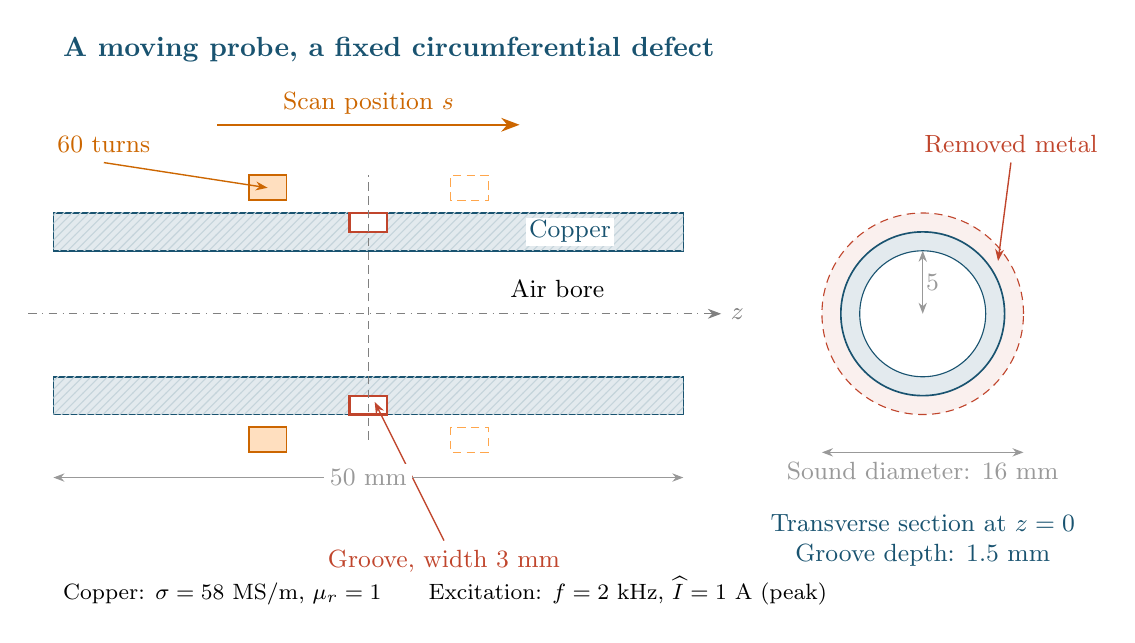
\begin{tikzpicture}[x=1.6mm,y=1.6mm,font=\small,
    dimension/.style={gray!80,{Stealth[length=1.4mm]}-{Stealth[length=1.4mm]}},
    leader/.style={line width=.5pt,-{Stealth[length=1.5mm]}},
    wall/.style={draw=ndtblue,fill=ndtblue!12,line width=.6pt},
    coil/.style={draw=orange!80!black,fill=orange!25,line width=.7pt}]
  \node[anchor=west,font=\bfseries,text=ndtblue] at (-25,21)
    {A moving probe, a fixed circumferential defect};
  % Full longitudinal section: the lower wall is the same revolved tube.
  \filldraw[wall] (-25,5) rectangle (25,8);
  \filldraw[wall] (-25,-8) rectangle (25,-5);
  \foreach \Side in {-1,1}{
    \fill[pattern=north east lines,pattern color=ndtblue!25]
      (-25,{\Side*5}) rectangle (25,{\Side*8});
    \filldraw[fill=white,draw=ndtred,line width=.8pt]
      (-1.5,{\Side*6.5}) rectangle (1.5,{\Side*8});
    \filldraw[coil] (-9.5,{\Side*9}) rectangle (-6.5,{\Side*11});
    \draw[orange!70,densely dashed]
      (6.5,{\Side*9}) rectangle (9.5,{\Side*11});
  }
  \draw[gray,dash dot,-Stealth] (-27,0)--(28,0) node[right] {$z$};
  \draw[gray,densely dashed] (0,-10)--(0,11);
  \draw[orange!80!black,thick,-Stealth] (-12,15)--(12,15)
    node[midway,above] {Scan position $s$};
  \draw[leader,orange!80!black] (-21,12) node[above] {60 turns}--(-8,10);
  \draw[leader,ndtred] (6,-18) node[below] {Groove, width 3 mm}--(.5,-7);
  \draw[dimension] (-25,-13)--(25,-13)
    node[midway,fill=white,inner sep=2pt] {50 mm};
  \node[text=ndtblue,fill=white,inner sep=1pt] at (16,6.5) {Copper};
  \node[fill=white,inner sep=1pt] at (15,2) {Air bore};
  % Transverse section through the defect. The dashed ring is the sound surface.
  \begin{scope}[shift={(44,0)}]
    \fill[ndtred!8] (0,0) circle[radius=8];
    \draw[ndtred,densely dashed] (0,0) circle[radius=8];
    \filldraw[wall] (0,0) circle[radius=6.5];
    \filldraw[fill=white,draw=ndtblue] (0,0) circle[radius=5];
    \draw[dimension] (0,0)--(0,5)
      node[midway,right,fill=white,inner sep=1pt] {5};
    \draw[leader,ndtred] (7,12) node[above] {Removed metal}--(35:7.3);
    \draw[dimension] (-8,-11)--(8,-11)
      node[midway,below] {Sound diameter: 16 mm};
    \node[align=center,text=ndtblue] at (0,-18)
      {Transverse section at $z=0$\\Groove depth: 1.5 mm};
  \end{scope}
  \node[anchor=west,font=\footnotesize] at (-25,-22)
    {Copper: $\sigma=58$ MS/m, $\mu_r=1$\qquad
     Excitation: $f=2$ kHz, $\widehat I=1$ A (peak)};
\end{tikzpicture}
\end{document}
